%% DOC: http://mirror.ctan.org/macros/latex/contrib/koma-script/scrguide.pdf
\documentclass[
	% DEFAULT: final, a4paper, 11pt
	twoside,
	DIV11,				% Seitengroesse (siehe scrguide.pdf)
	BCOR5mm,			% Zusaetzlicher Rand auf der Innenseite
	pagesize,			% Schreibt die Papiergroesse in die Datei, wichtig fuer Konvertierungen
	headsepline,		% Linie unter Kopfzeile
	parskip=half,		% Abstand zwischen zwei Abs�tzen
	bibtotoc,			% Bibliographie ins Inhaltsverzeichnis
	liststotoc,			% Abb.- und Tabellenverzeichnis ins Inhaltsverzeichnis
	cleardoubleempty	% Vakatseiten bleiben leer (etwa Seite vor einem Kapitel, das auf rechts beginnt)
]{scrbook}

%% Preambel
\usepackage[bottom=4cm, right=4cm]{geometry}

%~~~~~~~~~~~~~~~~~~~~~~~~~~~~~~
%% LOAD FIRST
%~~~~~~~~~~~~~~~~~~~~~~~~~~~~~~

%% Encoding
\usepackage[latin1]{inputenc}

%% Sprache
%  ftp://tug.ctan.org/pub/tex-archive/macros/latex/required/babel/babel.pdf
\usepackage[english]{babel}
\usepackage{blindtext}
%% Besserer Flattersatz (Linksbuendig, statt Blocksatz)
%  ftp://tug.ctan.org/pub/tex-archive/macros/latex/contrib/ms/ragged2e.pdf
\usepackage{ragged2e}

%% Bilder
%  ftp://tug.ctan.org/pub/tex-archive/macros/latex/required/graphics/grfguide.pdf
\usepackage[]{graphicx}

%% Farben
%  ftp://tug.ctan.org/pub/tex-archive/macros/latex/contrib/xcolor/xcolor.pdf
% Incompatible: Do not load when using pstricks !
\usepackage[table,usenames,dvipsnames]{xcolor} % Load for using rowcolors command in tables


%\usepackage[nointegrals]{wasysym}

%% Mathematik Basispaket
%  ftp://tug.ctan.org/pub/tex-archive/macros/latex/required/amslatex/math/amsldoc.pdf
\usepackage[]{amsmath}



% damit es nicht zu "no room for new \dimen"-Fehler kommt
\usepackage{etex}

\usepackage{tikz}
\usepackage{tkz-graph}
%  \usepackage{ifthen}
%  \usepackage{xstring}
%  \usepackage{calc}
%  \usepackage{pgfopts}

% See http://pgfplots.sourceforge.net/pgfplots.pdf
\usepackage{pgfplots}
\usepackage{pgfplotstable}
\usetikzlibrary{pgfplots.groupplots}
\usetikzlibrary{patterns}

% argument #1: any options
\newenvironment{customlegend}[1][]{%
    \begingroup
    % inits/clears the lists (which might be populated from previous
    % axes):
    \csname pgfplots@init@cleared@structures\endcsname
    \pgfplotsset{#1}%
}{%
    % draws the legend:
    \csname pgfplots@createlegend\endcsname
    \endgroup
}%

% makes \addlegendimage available (typically only available within an
% axis environment):
\def\addlegendimage{\csname pgfplots@addlegendimage\endcsname}

\usepackage{epstopdf}


%prevent number and text in list of figures to overlap
\makeatletter
\renewcommand*\l@figure{\@dottedtocline{1}{1.5em}{3em}}% 3em instead of 2.3em
\let\l@table\l@figure
\makeatother


%~~~~~~~~~~~~~~~~~~~~~~~~~~~~~~
%% TEXT
%~~~~~~~~~~~~~~~~~~~~~~~~~~~~~~

%% Schriftart

%% http://www.tug.dk/FontCatalogue/mathfonts.html



\usepackage{lmodern}
%\usepackage{kpfonts}
%\usepackage{mathptmx}
%\usepackage[sc]{mathpazo}
%\usepackage{charter}

\usepackage[T1]{fontenc}
%\usepackage{ae,aecompl}

%Optischer Randausgleich mit pdfTeX
\usepackage[%
	expansion=false, % if true: better typography, but larger PDF file (and not compatible with all fonts)
	protrusion=true
]{microtype}

%% Zum Unterstreichen
%  ftp://tug.ctan.org/pub/tex-archive/macros/latex/contrib/misc/ulem.sty
\usepackage[normalem]{ulem}

%%% Doc: ftp://tug.ctan.org/pub/tex-archive/macros/latex/contrib/soul/soul.pdf
\usepackage{soul}	% Unterstreichen, Sperren

%% Control the look & feel of the captions from floating environments like figure and table.
%  ftp://tug.ctan.org/pub/tex-archive/macros/latex/contrib/caption/caption.pdf
\usepackage{caption}
% Aussehen der Captions
\captionsetup{
   margin = 10pt,
   font = {small,rm},
   labelfont = {small,bf},
   format = plain, % oder 'hang'
   indention = 0em,  % Einruecken der Beschriftung
   labelsep = colon, %period, space, quad, newline
   justification = RaggedRight, % justified, centering
   singlelinecheck = true, % false (true=bei einer Zeile immer zentrieren)
   position = bottom %top
}
%%% Bugfix Workaround (Matthias Pospiech!?)
\DeclareCaptionOption{parskip}[]{}
\DeclareCaptionOption{parindent}[]{}

%% �berschriften komlett Umdefinieren
%  ftp://tug.ctan.org/pub/tex-archive/macros/latex/contrib/titlesec/titlesec.pdf
\usepackage{titlesec}

%% Mehrere Text-Spalten
\usepackage{multicol}

%%
% Doc: ftp://tug.ctan.org/pub/tex-archive/macros/latex/contrib/paralist/paralist.pdf
\usepackage{paralist}

%% Better than 'paralist' and 'enumerate' because it uses a keyvalue interface !
%  Do not load together with package 'enumerate'.
%  ftp://tug.ctan.org/pub/tex-archive/macros/latex/contrib/enumitem/enumitem.pdf
\usepackage{enumitem}

%% Schriftanpassung nach scrguide.pdf
\setkomafont{subsection}{\sffamily}

%% Chapter-Style definieren
% --> Rechtsb�ndig: Gro�e Kapitelnummer, darunter der Name
\titleformat{\chapter}[display]
{\filleft\usekomafont{chapter}\Huge}
{\fontsize{100pt}{50pt}\selectfont\thechapter}
{-2ex} %is vertical space in [display] mode
%Platz vor dem ganzen Krempel
{\vspace{1ex}} %1ex ist die H�he von x im aktuellen Font
%Platz danach
[\vspace{1ex}]


\usepackage{nowidow}


%~~~~~~~~~~~~~~~~~~~~~~~~~~~~~~
%% TABELLEN (tabularx wird von ltxtable geladen!?)
%~~~~~~~~~~~~~~~~~~~~~~~~~~~~~~

%% Tabellen ueber mehere Seiten
%  ftp://tug.ctan.org/pub/tex-archive/macros/latex/contrib/carlisle/ltxtable.pdf
\usepackage{ltxtable} % Longtable + tabularx
                      % (multi-page tables) + (auto-sized columns in a fixed width table)
%% bessere Abstaende innerhalb der Tabelle (Layout))
%  ftp://tug.ctan.org/pub/tex-archive/macros/latex/contrib/booktabs/booktabs.pdf
\usepackage{booktabs}

%% Erweiterte Funktionen innerhalb von Tabellen
%  ftp://tug.ctan.org/pub/tex-archive/macros/latex/contrib/multirow/multirow.sty
\usepackage{multirow} % Mehrfachspalten

%% Tabellen: Ausrichtung an Komma oder Punkt
\usepackage{dcolumn}

\usepackage{pbox}
\usepackage{footnote}

%~~~~~~~~~~~~~~~~~~~~~~~~~~~~~~
%% FARBEN
%~~~~~~~~~~~~~~~~~~~~~~~~~~~~~~

\definecolor{sectioncolor}{RGB}{0, 0, 0}    % Schwarz

% Farbe des Textes
\definecolor{textcolor}{RGB}{0, 0, 0}        % Schwarz

% Farbe fuer grau hinterlegte Boxen (fuer Paket framed.sty)
\definecolor{shadecolor}{gray}{0.90}

% Farben fuer die Links im PDF
\definecolor{pdfurlcolor}{rgb}{0.6,0,0}
\definecolor{pdffilecolor}{rgb}{0,0.4,0}
\definecolor{pdflinkcolor}{rgb}{0,0,0.75}

% Java Syntax Highlighting
\definecolor{javared}{rgb}{0.6,0,0} % for strings
\definecolor{javagreen}{rgb}{0.25,0.5,0.35} % comments
\definecolor{javapurple}{rgb}{0.5,0,0.35} % keywords
\definecolor{javadocblue}{rgb}{0.25,0.35,0.75} % javadoc

% more
\definecolor{darkblue}{rgb}{0.0,0.0,0.6}
\definecolor{cyan}{rgb}{0.0,0.6,0.6}

%colors for teh dbs
\colorlet{EventStoreClr}{SpringGreen}
\colorlet{HBaseClr}{Dandelion}
\colorlet{PostgresClr}{Cyan}
\colorlet{RedisClr}{Apricot}


\definecolor{plot1}{RGB}{128,0,128}
\definecolor{plot2}{RGB}{128,128,128}
\definecolor{plot3}{RGB}{236,217,198}
\definecolor{plot4}{RGB}{255,178,178}
\definecolor{plot5}{RGB}{178,178,255}



%~~~~~~~~~~~~~~~~~~~~~~~~~~~~~~
%% LITERATUR
%~~~~~~~~~~~~~~~~~~~~~~~~~~~~~~

% ftp://tug.ctan.org/pub/tex-archive/macros/latex/contrib/natbib/natbib.pdf
%\usepackage[%
	%round,	%(default) for round parentheses;
%	square,	% for square brackets;
	%curly,	% for curly braces;
	%angle,	% for angle brackets;
	%colon,	% (default) to separate multiple citations with colons;
%	comma,	% to use commas as separaters;
	%authoryear,% (default) for author-year citations;
%	numbers,	% for numerical citations;
	%super,	% for superscripted numerical citations, as in Nature;
%	sort,		% orders multiple citations into the sequence in which they appear in the list of references;
%	sort&compress,    % as sort but in addition multiple numerical citations
                   % are compressed if possible (as 3-6, 15);
	%longnamesfirst,  % makes the first citation of any reference the equivalent of
                   % the starred variant (full author list) and subsequent citations
                   %normal (abbreviated list);
	%sectionbib,      % redefines \thebibliography to issue \section* instead of \chapter*;
                   % valid only for classes with a \chapter command;
                   % to be used with the chapterbib package;
	%nonamebreak,     % keeps all the authors names in a citation on one line;
                   %causes overfull hboxes but helps with some hyperref problems.
%]{natbib}

%% Bibliography styles created with custombib
%  ftp://tug.ctan.org/pub/tex-archive/macros/latex/contrib/custom-bib/makebst.pdf
%\bibliographystyle{bib/bst/AlphaDINFirstName}
\bibliographystyle{alpha}


%~~~~~~~~~~~~~~~~~~~~~~~~~~~~~~
%% BILDER & GRAFIKEN
%~~~~~~~~~~~~~~~~~~~~~~~~~~~~~~

% Stellt die Option [H] fuer Floats zur Verf�gung
\usepackage{float}

% Floats immer erst nach der Referenz setzen
\usepackage{flafter}
 
%% Platz ober- und unterhalb des Bildes
\setlength{\intextsep}{0.5\baselineskip} 

%%% Doc: http://www.ctan.org/tex-archive/macros/latex/contrib/sidecap/sidecap.pdf
\usepackage[%
%	outercaption,%	(default) caption is placed always on the outside side
%	innercaption,% caption placed on the inner side
%	leftcaption,%  caption placed on the left side
	rightcaption,% caption placed on the right side
%	wide,%			caption of float my extend into the margin if necessary
%	margincaption,% caption set into margin
	ragged,% caption is set ragged
]{sidecap}

\renewcommand\sidecaptionsep{2em}
%\renewcommand\sidecaptionrelwidth{20}
\sidecaptionvpos{table}{c}
\sidecaptionvpos{figure}{c}

%% Subfigures
%  ftp://tug.ctan.org/pub/tex-archive/macros/latex/contrib/subfig/subfig.pdf
%  Incompatible: loads package capt-of. Loading of 'capt-of' afterwards will fail therefor
\usepackage{subfig}

% Aussehen der Captions fuer subfigures (subfig-Paket)
\captionsetup[subfloat]{%
   margin = 10pt,
   font = {small,rm},
   labelfont = {small,bf},
   format = plain, % oder 'hang'
   indention = 0em,  % Einruecken der Beschriftung
   labelsep = space, %period, space, quad, newline
   justification = RaggedRight, % justified, centering
   singlelinecheck = true, % false (true=bei einer Zeile immer zentrieren)
   position = bottom, %top
   labelformat = parens % simple, empty % Wie die Bezeichnung gesetzt wird
}

%% Bilder von Text Umfliessen lassen
%  ftp://tug.ctan.org/pub/tex-archive/macros/latex/contrib/wrapfig/wrapfig.sty
% defines wrapfigure and wrapfloat
\usepackage{wrapfig}

% Platz ober- und unterhalb des Bildes
\setlength{\intextsep}{0.5\baselineskip} 
%\setlength{\wrapoverhang}{\marginparwidth} % Overlap des Bildes ...
%\addtolength{\wrapoverhang}{\marginparsep} % ... in den margin
%\setlength{\columnsep}{1em} % Abstand zum Text

% Make float placement easier ???
\renewcommand{\floatpagefraction}{.75} % vorher: .5
\renewcommand{\textfraction}{.1}       % vorher: .2
\renewcommand{\topfraction}{.8}        % vorher: .7
\renewcommand{\bottomfraction}{.5}     % vorher: .3
\setcounter{topnumber}{3}              % vorher: 2
\setcounter{bottomnumber}{2}           % vorher: 1
\setcounter{totalnumber}{5}            % vorher: 3

%%% Doc: http://www.ctan.org/tex-archive/macros/latex/contrib/sidecap/sidecap.pdf
\usepackage[%
%	outercaption,%	(default) caption is placed always on the outside side
%	innercaption,% caption placed on the inner side
%	leftcaption,%  caption placed on the left side
	rightcaption,% caption placed on the right side
%	wide,%			caption of float my extend into the margin if necessary
%	margincaption,% caption set into margin
	ragged,% caption is set ragged
]{sidecap}

\renewcommand\sidecaptionsep{2em}
%\renewcommand\sidecaptionrelwidth{20}
\sidecaptionvpos{table}{c}
\sidecaptionvpos{figure}{c}


%~~~~~~~~~~~~~~~~~~~~~~~~~~~~~~
%% KOPF- UND FUSSZEILEN
%~~~~~~~~~~~~~~~~~~~~~~~~~~~~~~

% ftp://tug.ctan.org/pub/tex-archive/macros/latex/contrib/koma-script/scrguide.pdf
\usepackage[%
   automark,         % automatische Aktualisierung der Kolumnentitel
   nouppercase,      % Grossbuchstaben verhindern
   %markuppercase    % Grossbuchstaben erzwingen
   %markusedcase     % vordefinierten Stil beibehalten
   %komastyle,       % Stil von Koma Script
   %standardstyle,   % Stil der Standardklassen
]{scrpage2}

\renewcommand*{\chaptermark}[1]{%
  \markboth{\chaptermarkformat #1}{}}
\renewcommand*{\sectionmark}[1]{%
  \markright{\sectionmarkformat #1}}


%~~~~~~~~~~~~~~~~~~~~~~~~~~~~~~
%% MATHE & FORMELN
%~~~~~~~~~~~~~~~~~~~~~~~~~~~~~~

%% Bracket Schreibweise
%  ftp://tug.ctan.org/pub/tex-archive/macros/latex/contrib/misc/braket.sty
\usepackage{braket}

%% Durchstreichen
%  ftp://tug.ctan.org/pub/tex-archive/macros/latex/contrib/misc/cancel.sty
\usepackage{cancel}

%% Hervorheben
%  ftp://tug.ctan.org/pub/tex-archive/macros/latex/contrib/mh/doc/empheq.pdf
\usepackage{empheq}


%~~~~~~~~~~~~~~~~~~~~~~~~~~~~~~
%% LISTINGS & CODE & DIAGRAMME (UML)
%~~~~~~~~~~~~~~~~~~~~~~~~~~~~~~

%% Listings Paket
%  http://www.pvv.ntnu.no/~berland/latex/docs/listings.pdf
\usepackage{listings}
\lstloadlanguages{Java,SQL,XML}

%% f�r alle Listings
\lstset{ 
		 backgroundcolor=\color{gray!12},
         basicstyle=\footnotesize\ttfamily, % Standardschrift    
         numbers=left,               % Ort der Zeilennummern
         numberstyle=\tiny,          % Stil der Zeilennummern
%         stepnumber=1,               % Abstand zwischen den Zeilennummern
         numbersep=5pt,              % Abstand der Nummern zum Text
         tabsize=2,                  % Groesse von Tabs
         extendedchars=true,         %
         breaklines=true,            % Zeilen werden Umgebrochen    
         showspaces=false,           % Leerzeichen anzeigen ?%         showtabs=false,             % Tabs anzeigen ?
         showstringspaces=false,     % Leerzeichen in Strings anzeigen ?
		 %frame=single,
		 %frame={l,r,b},
		 rulecolor=\color{black!60},
		 %captionpos=b,
		 xleftmargin=15pt,
		 framexleftmargin=14pt,
		 %framexrightmargin=4pt,
         %framexbottommargin=4pt,
         %framextopmargin=4pt,
         belowcaptionskip=5pt,
 }
 
\DeclareCaptionFont{white}{\color{white}}
\DeclareCaptionFormat{listing}{\colorbox{black!60}{\parbox{0.985\textwidth}{\hspace{13pt}#1#2#3}}}
\captionsetup[lstlisting]{format=listing,labelfont={white},textfont={sf,white},
singlelinecheck=false, margin=1pt, font={bf,small}}

\lstdefinestyle{Java}
{
  keywordstyle=\color{javapurple}\bfseries,
  stringstyle=\color{javared}, % Farbe der String
  commentstyle=\color{javagreen}, % Farbe der Kommentare
  morecomment=[s][\color{javadocblue}]{/**}{*/},
  morekeywords={public,lang}
}

\lstdefinelanguage{XML}
{
  morestring=[b][\color{javadocblue}]",
  morestring=[s][\color{black}]{>}{<},
  %morecomment=[s]{<?}{?>},
  %stringstyle=\color{javadocblue},
  identifierstyle=\color{javagreen},
  keywordstyle=\color{javapurple},
  morekeywords={category,lang}% list your attributes here
}

%% tikz-uml zur Darstellung von UML-Diagrammen
%  http://www.ensta-paristech.fr/~kielbasi/tikzuml/index.php?lang=en
\usepackage{packages/tikz-uml}	% aus dem Ordner packages, da nicht im MikTex-Repository!

%~~~~~~~~~~~~~~~~~~~~~~~~~~~~~~
%% SONSTIGES
%~~~~~~~~~~~~~~~~~~~~~~~~~~~~~~

\setcounter{lofdepth}{1}  % Tiefe Abbildungsverzeichnis, 1 = nur figures, 2 = figures + subfigures
\setcounter{secnumdepth}{2}    % Tiefe der Nummerierung
\setcounter{tocdepth}{2}	   % Tiefe Inhaltsverzeichnis

%% Intelligente Querverweise
%  http://www.ctex.org/documents/packages/bibref/varioref.pdf
\usepackage[english]{varioref}

%% Fussnoten/Endnoten
%  ftp://tug.ctan.org/pub/tex-archive/macros/latex/contrib/footmisc/footmisc.pdf
\usepackage[
   bottom,      % Footnotes appear always on bottom. This is necessary
                % especially when floats are used
   stable,      % Make footnotes stable in section titles
   perpage,     % Reset on each page
   %para,       % Place footnotes side by side of in one paragraph.
   %side,       % Place footnotes in the margin
   ragged,      % Use RaggedRight
   %norule,     % suppress rule above footnotes
   multiple,    % rearrange multiple footnotes intelligent in the text.
   %symbol,     % use symbols instead of numbers
]{footmisc}

%% Advanced features for clever quotations
%  ftp://tug.ctan.org/pub/tex-archive/macros/latex/contrib/csquotes/csquotes.pdf
\usepackage[%
   babel,            % the style of all quotation marks will be adapted
                     % to the document language as chosen by 'babel'
   german=quotes,		% Styles of quotes in each language
   english=british,
   french=guillemets
]{csquotes}

\renewcommand*{\mkblockquote}[4]{\enquote{#1}#2#4#3}


% Use �\cite{NEEDED}� to get Wikipedia-style �citation needed� in document
\usepackage{ifthen}
\let\oldcite=\cite
\renewcommand\cite[1]{\ifthenelse{\equal{#1}{NEEDED}}{\ensuremath{^\texttt{\color{red}[citation~needed]}}}{\oldcite{#1}}}

%\usepackage[disable]{todonotes}
\usepackage{todonotes}

% margin notes aligned with paragraph
\newcommand{\mnote}[1]{{\hspace{0pt}\marginpar[\raggedleft\emph{\small{#1}}]{\raggedright\emph{\small{#1}}}}\ignorespaces}


%~~~~~~~~~~~~~~~~~~~~~~~~~~~~~~
%% LINKS (hyperref am Besten zum Schluss Laden laut Doku)
%~~~~~~~~~~~~~~~~~~~~~~~~~~~~~~

%% Setzen von URLs. In Verbindung mit hyperref sind diese auch aktive Links.
%  ftp://tug.ctan.org/pub/tex-archive/macros/latex/contrib/misc/url.sty
\usepackage{url}
\urlstyle{sf}

%% Basispaket hyperref
%  ftp://tug.ctan.org/pub/tex-archive/macros/latex/contrib/hyperref/doc/manual.pdf
\usepackage[
   % Farben fuer die Links
   colorlinks=false,%true,         % Links erhalten Farben statt Kaeten
   urlcolor=pdfurlcolor,    % \href{...}{...} external (URL)
   filecolor=pdffilecolor,  % \href{...} local file
   linkcolor=pdflinkcolor,  %\ref{...} and \pageref{...}
   citecolor=pdffilecolor,	% Farbe von Links zum Literaturverzeichnis
   % Links
   raiselinks=true,			% calculate real height of the link
   breaklinks,              % Links �berstehen Zeilenumbruch
   backref=page,            % Backlinks im Literaturverzeichnis (section, slide, page, none)
   pagebackref=true,        % Backlinks im Literaturverzeichnis mit Seitenangabe
   verbose,					% extra diagnostic messages are printed in the log file
   hyperindex=true,         % backlinkex index
   linktocpage=true,        % Inhaltsverzeichnis verlinkt Seiten
   hyperfootnotes=false,    % Keine Links auf Fussnoten
   % Bookmarks
   bookmarks=true,          % Erzeugung von Bookmarks fuer PDF-Viewer
   bookmarksopenlevel=1,    % Gliederungstiefe der Bookmarks
   bookmarksopen=true,      % Expandierte Untermenues in Bookmarks
   bookmarksnumbered=true,  % Nummerierung der Bookmarks
   bookmarkstype=toc,       % Art der Verzeichnisses
   % Anchors
   plainpages=false,        % Anchors even on plain pages ?
   pageanchor=true,         % Pages are linkable
   % PDF Informationen
   pdftitle={},             % Titel
   pdfauthor={},            % Autor
   pdfcreator={LaTeX, hyperref, KOMA-Script}, % Ersteller
   %pdfproducer={pdfeTeX 1.10b-2.1} %Produzent
   pdfstartview=FitH,       % Dokument wird Fit Width geaefnet
   pdfpagemode=UseOutlines, % Bookmarks im Viewer anzeigen
   pdfpagelabels=true      % set PDF page labels
]{hyperref}

%% Links auf Gleitumgebungen springen nicht zur Beschriftung, sondern zum Anfang der Gleitumgebung
%  ftp://tug.ctan.org/pub/tex-archive/macros/latex/contrib/oberdiek/hypcap.pdf
\usepackage[all]{hypcap}

%% Erweitert Angabe eines Zitats (im Literaturverzeichnis)
\renewcommand*{\backrefalt}[4]{%
   	% alternative interface
   	% #1: number of distinct back references
   	% #2: backref list with distinct entries
   	% #3: number of back references including duplicates
   	% #4: backref list including duplicates
   	\ifnum#1>0 %
	   	\mbox{(cited on %
	   	\ifnum#1=1 %
			   page~%
		   \else
	   		pages~%
	   	\fi
	   	#2)}%
   	\fi
   }

   
  


%% Commands
%% Document Information
\newcommand{\infoInstitute}{Rheinische Friedrich-Wilhelms-Universit�t Bonn}
\newcommand{\infoDepartment}{Institute of Computer Science III}
\newcommand{\infoAdvisor}{Jun.-Prof. Dr. Alexander Markowetz}
\newcommand{\infoTitleHead}{Menthal}
\newcommand{\infoTitle}{Distributed online processing of big data streams}
\newcommand{\infoThesisType}{Master's Thesis}
\newcommand{\infoAuthorP}{Svetlana Pospelova}
\newcommand{\infoAuthorI}{Viacheslav Inozemtsev}
\newcommand{\infoAuthor}{\infoAuthorP \textsc{ }\textsc{ }\textsc{ }\infoAuthorI}
\newcommand{\infoMatriculationP}{2551566}
\newcommand{\infoMatriculationI}{2544488}
\newcommand{\infoLocation}{Bonn}
\newcommand{\infoDate}{June 19, 2014}

%% New Commands
\newcommand{\package}[1]{\texttt{\itshape#1}}
\newcommand{\command}[1]{\texttt{#1}}
\newcommand{\env}[1]{\texttt{#1}}

%include author in section title in a flexible way
\newcommand{\authorsection}[2]{
\ifx&#2&%
  % #2 is empty
  \section{#1 \color{red}{NO AUTHOR}}
\else
  \section{#1 \small[#2]}
\fi
}


% \newcommand{\authorsection}[2]{
%    \section{#1$_{#2}$}}
%% Kommandos fuer Tabellen. Entnommen aus The LateX Companion, tabsatz.ps und diversen Dokus:

%%% ---| Farben fuer Tabellen |-------------------

\colorlet{tablesubheadcolor}{gray!30}
\colorlet{tableheadcolor}{gray!25}
\colorlet{tableblackheadcolor}{black!100}
\colorlet{tablerowcolor}{gray!10.0}

%%% ---------------------------------------------


%%% -| Neue Spaltendefinitionen 'columntypes' |--
%
% Belegte Spaltentypen:
% l - links
% c - zentriert
% r - rechts
% p,m,b  - oben, mittig, unten
% X - tabularx Auto-Spalte

% um Tabellenspalten mit Flattersatz zu setzen, muss \\ vor
% (z.B.) \raggedright geschuetzt werden:
\newcommand{\PreserveBackslash}[1]{\let\temp=\\#1\let\\=\temp}


% Spalten mit Flattersatz und definierte Breite:
% m{} -> mittig
% p{} -> oben
% b{} -> unten
%
% Linksbuendig:
\newcolumntype{v}[1]{>{\PreserveBackslash\RaggedRight\hspace{0pt}}p{#1}}
\newcolumntype{M}[1]{>{\PreserveBackslash\RaggedRight\hspace{0pt}}m{#1}}
% % Rechtsbuendig :
% \newcolumntype{R}[1]{>{\PreserveBackslash\RaggedLeft\hspace{0pt}}m{#1}}
% \newcolumntype{S}[1]{>{\PreserveBackslash\RaggedLeft\hspace{0pt}}p{#1}}
% % Zentriert :
% \newcolumntype{Z}[1]{>{\PreserveBackslash\Centering\hspace{0pt}}m{#1}}
% \newcolumntype{A}[1]{>{\PreserveBackslash\Centering\hspace{0pt}}p{#1}}

\newcolumntype{Y}{>{\PreserveBackslash\RaggedLeft\hspace{0pt}}X}
%%% Spalten fuer Mathematik
%
% serifenlose Matheschrift
\newcolumntype{s}[1]{%
	>{\DC@{.}{,}{#1}\mathsf\bgroup}l%
	<{\egroup\DV@end}%
}

% Tabellenspaltentyp fuer den Kopf: (Farbe + Ausrichtung)
\newcolumntype{H}[1]{>{\columncolor{tableheadcolor}}l}

% aequivalent aus typokurz (fett+grau+links)
% \newcolumntype{H}{>{\fontseries{b}\selectfont%
%     \columncolor[gray]{.8}[6pt][0pt]}l}
%%% --------------------------------------------


%%% ---|Listen in Tabellen |--------------------
\newcommand{\removeindentation}{%
	\leftmargini=\labelsep%
	\advance\leftmargini by \labelsep%
}
%
\makeatletter
\newcommand\tableitemize{
	\@minipagetrue%
	\removeindentation
}
\makeatother
%%% --------------------------------------------

%%% ---|Layout der Tabellen |-------------------

% Neue Umgebung fuer Tabellen:

\newenvironment{Tabelle}[2][c]{%
  \tablestylecommon
  \begin{longtable}[#1]{#2}
  }
  {\end{longtable}%
  \tablerestoresettings
}


% Groesse der Schrift in Tabellen
\newcommand{\tablefontsize}{ \footnotesize}
\newcommand{\tableheadfontsize}{\footnotesize}

% Layout der Tabelle: Ausrichtung, Schrift, Zeilenabstand
\newcommand\tablestylecommon{%
  \renewcommand{\arraystretch}{1.4} % Groessere Abstaende zwischen Zeilen
  \normalfont\normalsize            %
  \sffamily\tablefontsize           % Serifenlose und kleine Schrift
  \centering %                       % Tabelle zentrieren
}

\newcommand{\tablestyle}{
	\tablestylecommon
	%\tablealtcolored
}

% Ruecksetzten der Aenderungen
\newcommand\tablerestoresettings{%
  \renewcommand{\arraystretch}{1}% Abstaende wieder zuruecksetzen
  \normalsize\rmfamily % Schrift wieder zuruecksetzen
}

% Tabellenkopf: Serifenlos+fett+schraeg+Schriftfarbe
\newcommand\tablehead{%
  \tableheadfontsize%
  \sffamily\bfseries%
  %\slshape
  %\color{white}
}

\newcommand\tablesubheadfont{%
  \tableheadfontsize%
  \sffamily\bfseries%
  \slshape
  %\color{white}
}


\newcommand\tableheadcolor{%
	%\rowcolor{tablesubheadcolor}
	%\rowcolor{tableblackheadcolor}
	\rowcolor{tableheadcolor}%
}

\newcommand\tablesubheadcolor{%
	\rowcolor{tablesubheadcolor}
	%\rowcolor{tableblackheadcolor}
}


\newcommand{\tableend}{\arrayrulecolor{black}\hline}

% Tabellenkopf (1=Spaltentyp, 2=Text)
% \newcommand{\tablehead}[2]{
%   \multicolumn{1}{#1@{}}{%
%     \raisebox{.1mm}{% Ausrichtung der Beschriftung
%       #2%
%     }\rule{0pt}{4mm}}% unsichtbare Linie, die die Kopfzeile hoeher macht
% }


\newcommand{\tablesubhead}[2]{%
  \multicolumn{#1}{>{\columncolor{tablesubheadcolor}}l}{\tablesubheadfont #2}%
}

% Tabellenbody (=Inhalt)
\newcommand\tablebody{%
\tablefontsize\sffamily\upshape%
}

\newcommand\tableheadshaded{%
	\rowcolor{tableheadcolor}%
}
\newcommand\tablealtcolored{%
	\rowcolors{1}{tablerowcolor}{white!100}%
}
%%% --------------------------------------------

\newlength{\mylen}
\newlength{\adjusthspace}

\newenvironment{tabularc}[2]
{%
	\setlength\mylen{#2/(#1)-\tabcolsep*2-\arrayrulewidth*(#1+1)/(#1)}%
	%\setlength{\adjusthspace}{((#2-1)/2)*\linewidth}
	%\par\noindent
	%\hspace*{-\the\adjusthspace}
	\begin{tabular}%{#2}%
		{*{#1}{v{\the\mylen}}}%
}
{\end{tabular}\par}


%% Silbentrennung
\hyphenation{}


%% DOKUMENT
\begin{document}

\pagenumbering{gobble}	% turn off page numbering
%\sloppy		% Schaltet auf eine gro�z�gige Formatierungsweise um, die relativ wenige Worttrennungen
				% am Zeilenende erzeugt, daf�r aber auch etwas gr��ere Wortabst�nde innerhalb der Zeilen zul��t.

%% Titel
\newgeometry{margin=2cm, left=2.5cm}
\begin{titlepage}
	\centering
	
	% HEAD
	\Large\scshape
	\infoInstitute\\
	\infoDepartment
	\vspace{0.17\textheight}\\
	
	% TITLE
	\Huge\normalfont
	\infoTitleHead
	\vspace{0.3\baselineskip}\\
	\huge\bfseries
	\infoTitle
	\vspace{0.12\textheight}\\
	
	% TYPE AND ADVISOR
	\Large
	\infoThesisType\\[0.3\baselineskip]
	\normalfont\large
	Supervisor:	\infoAdvisor
	\vspace{4\baselineskip}\\
	
	% AUTHOR
	\Large
	%\hspace{50pt}
	\infoAuthorP
	
	\infoAuthorI
	%\hspace{85pt}
	%\infoAuthor \\[0.3\baselineskip]
	%\large
	%Matrikelnummer \infoMatriculation
	\vspace{4\baselineskip}\\
	\infoLocation, \infoDate
	\vfill
	
	% LOGO
	
\includegraphics[width=0.4\textwidth]{images/uni_bonn_logo}
	
\end{titlepage}
\restoregeometry


\chapter*{Decleration of Authorship}

I hereby certify that my part of this thesis, indicated by my initials, has been composed by me and is based on my own work, unless stated otherwise.
No other person's work has been used without due acknowledgement in this thesis.
All references and verbatim extracts have been quoted.
Every source of information, including graphs and data sets, has been specifically acknowledged.
\vspace{4\baselineskip}\\
\infoLocation, \infoDate \hfill \infoAuthor
\vspace{4\baselineskip}\\

\chapter*{}
\vfill
\rule{\textwidth}{0.4pt}
\emph{``Any sufficiently advanced technology is indistinguishable from magic.''}\\ Arthur C. Clarke

%% Inhaltsverzeichnis
\frontmatter		% preface (roman numbering)
\tableofcontents

%% Inhalt


\mainmatter			% arabic numbering for content
\pagestyle{scrheadings}
\clearscrheadfoot
\chead{\leftmark \hfill \rightmark}
\cfoot[\pagemark]{\pagemark}
\chapter{Introduction}
\label{chap:introduction}

In the good old times, when we had hard disk drives of just several gigabytes, it was easy to write a program and do any kind of manipulations with the data, that were at the disposal.
Back then we built a model, and decided what data we need to have, to make the model functioning.
For example, if you had a company, it was easy to devise ER-model and to build a database with corresponding tables, that would be stored on a single machine.
It would possible have a slave machine, that repeated the whole database for a case of failure.
In the normal case we would simply do a dump of the database once in week.
All selects were fast and pretty, and nobody thought about need to make things scalable.
We used only data that were necessary to maintain the company's meta information.

Nowdays everything has changed.
We now have immense amount of data coming from everywhere.
Hard disks are large, and get larger.
They even evolved to solid state drives without any mechanical parts, and became hence much faster.
Such environment has brought us to a completely different way of thinking.

We keep everything!
This is our motto.
There is no necessity any more to think about space, because it has become so cheap.
We can store everything possible storable, and then answer any kind of queries later on, when they arise.
Such model can in theory provide much more information for a final client, but it has its drawback.
All the methods of storage and computations have to be reinvented.
We cannot anymore store everything on the single machine in the single relational database.

\mnote{Big Data}
To overcome this problem the whole new branch of computer science and information technology has appeared - \textit{Big Data}.
This is a very broad term, that encompasses different topics as for example storage systems, data processing systems, cloud computing, etc.
All these systems, no matter do they store data or do some processing, have one thing in common - \textit{distributivity}.
Data storage systems in the big data context are usually cold \textit{noSQL} databases, because they have different data storing models comparing to relational databases.
They lay on many machines and provide reliability of data, so that if one machine dies, data remains alive.
Data processing systems use many machines to do computations.
Processing model is so, that it is easy to add new machines and increase speed of processing almost linearly.
These systems also provide reliability in the sense, that all the data is always processed in the end, no matter what happens in the meantime with machines used for computing.

One of the ideas that arised in the depths of the Institute of Computer Science of the University of Bonn was to measure usage of smartphones by their owners.
Menthal is a group, that works on this project.
It created an application for Android operating system, that gathers and sends data about use of smartphone to the server, where different computations are being made.
Important to mention, that no private data is ever sent, only different markers (numbers) about how often a person unlock the phone, launches a particular app, and so on.
As the bottom line, this emerged to a real big data system, where large amounts of data are being gathered continuously, and many different questions can be answered using this data.

The classical approach of data processing and big data architecture was bacth processing.
It means we gather data, and once in a while we do all computations we need to produce relevant results for query answering.
Then we can answer any particular question easily.
But it has become recently not enough, because the delay of the batch computations is too big.
It can take hours or event days.
In general, it is important to maintain the system in such state, that it can answer any specific query right away having the most relevant results ready.

Here the online processing comes out of the scene, and we need to thing about how to answer with low latency to the query, that client of the system has.
Low latency means that we must provide a time guarantee, that data, that has come, will be in the query answers not later from its coming time, than this guarantee.


Lambda architecture as a solution, combining batch and online processing

our system
\chapter{The Menthal Story}
\label{chap:menthal_story}
Such devices as smartphones became an integral part of modern life.
People use it not only for communication, but for plenty of other purposes, like reading books, surfing in the Internet, playing games, etc.
However, most of the users can not correctly estimate the time spent on their phone during the day.
Besides, information about how people use their phones can be analysed from different sides.
Psychological research, statistical calculations, medicine and healthcare projects, advertising - these are several examples of where such data can yield a profit.
Menthal is an application that is designed specifically for these purposes.
This chapter describes the main functionality and technical details of this application.

Nowadays mobile/smartphone excessive usage becomes a critical problem.
People constantly use these devices, making calls, sending messages, surfing in the Internet or just playing.
People are distracted by their phones even on personal meetings, parties and dates.
When a person leaves his phone at home, quite often he feels nervous and irritated.
Some people suffer from a cellphone vibration syndrome, when one feels as if a cellphone is vibrating but in fact it is not.
Sometimes they unlock the phone and check messages or social network pages unconsciously, just to make sure that nothing new has happened. 

The crucial problem is that people are not able to detect that they concentrate on their smartphones too much.
Few of them can correctly estimate the daily usage period of the device.
First, it is difficult to evaluate yourself, take a detached view on your behavior.
For example, one can unlock his phone 45 times per day and use it for 2 minutes on average.
However, in the end of the day it sums up to 1,5 hours.
This fact can surprise the user, because his estimated frequency of interaction with a phone and usage time would be much smaller.
Second, even if a person can correctly assess the wasted time, it is morally unpleasant to confirm these figures.
For instance, one plays a game on his smartphone instead of working on important task that has to be accomplished.
Finally, the task is not finished, the person realizes that the reason was that mobile game, but it is easier to say that there was not enough time to complete the task.  
Thus, exterior assessment mechanism is needed to calculate how much time a user spend on his smartphone, what applications he uses and when.    

At the same time, there is no proper study how people use their phones.
Currently most of the researches in the field of human-smartphone interaction involve direct interaction with a user group, by means of questionnaires and interviews.
Recently special software applications for smartphones to keep track of user actions emerge.
However, they still require the interaction with users, showing dialogue boxes and asking questions.
It introduces a certain bias into the results of the research, because a user gets distracted by this interference.
Only an application that is invisible for users can help to make a complete and thorough research.

The results of human-smartphone study can be used in various fields.
For example, France introduces a rule to switch off work phones after 18:00 and till 9:00, to protect employees from official duties outside office hours.
To perform such introduction, it is important to investigate how people of various professions use their work phone.
This research can help to detect the cases when it is actually necessary to block the phones.
In some cases maybe it is sufficient to block only particular functions, such as emails or text messages.

Moreover, it is essential to determine how people use their smartphones to make user-friendly application interfaces. 
An application interface has a big influence on user.
Developers can make it attractive and handy, that encourages users to use the application again even if there is no actual necessity.
If a person wants to decrease the time spent on the smartphone, a special enhanced interface can help.
For example, the phone can warn user when he spends too much time using the device during the day.  

As a result, there are two problems that have to be solved. 
On the one hand, there is a need to provide a user with his smartphone use information.
On the other hand, it is necessary to supply researches with a tool that tracks smartphone usage.
Menthal, an application for smartphones, combines these two features and provides solutions for both of these problems. 

\authorsection{Study}{SP}
Menthal is an application that gathers phone usage data and stores it on a server for further analysis, providing user with a feedback.
Phone usage data includes the number of times user unlocks his phone, the number of performed calls and sent SMS, etc.
The user receives a feedback about the smartphone usage statistics that is provided by the server.
In this case Menthal uses the same concept as Google: it grants users a free service in return to data.
This approach works well, and the high number of Menthal users demonstrates it. 

Prior to present Menthal application a pilot study was conducted. 
It was a psychological experiment on 49 participants.
During 5 weeks their telephone/SMS usage was measured by means of a mobile phone application.
The personality dimensions were determined using questionnaire.
The goal of this study was to detect a connection between smartphone usage patterns and personality traits.

In contrast to other similar attempts, this work uses automatized approach for gathering information instead of self-report data.
The application tracks tuples for calls of the format (anonymized number, start time, end time, in/out).
SMS tuples have a form (anonymized number, length of the message, time sent for outgoing messages / time received, time read for incoming SMS).
The application is not visible for the user, uploading data to the server automatically.
Later collected data is analysed on the server in the context of personality traits.
Among the result of the study one can observe a positive correlation between extraversion and the number and frequency of telephone calls.

\authorsection{Technical details}{SP}
This experiment develops into an independent smartphone application for mass usage. 
It collects data, providing user with a feedback and supplying psychologists with information that can be analysed later on.
Figure~\ref{fig:menthal_architecture} illustrates the Menthal architecture.
The application includes a client and a server part, that interact with each other via HTTPS.

\begin{figure}[h]
  \centering
  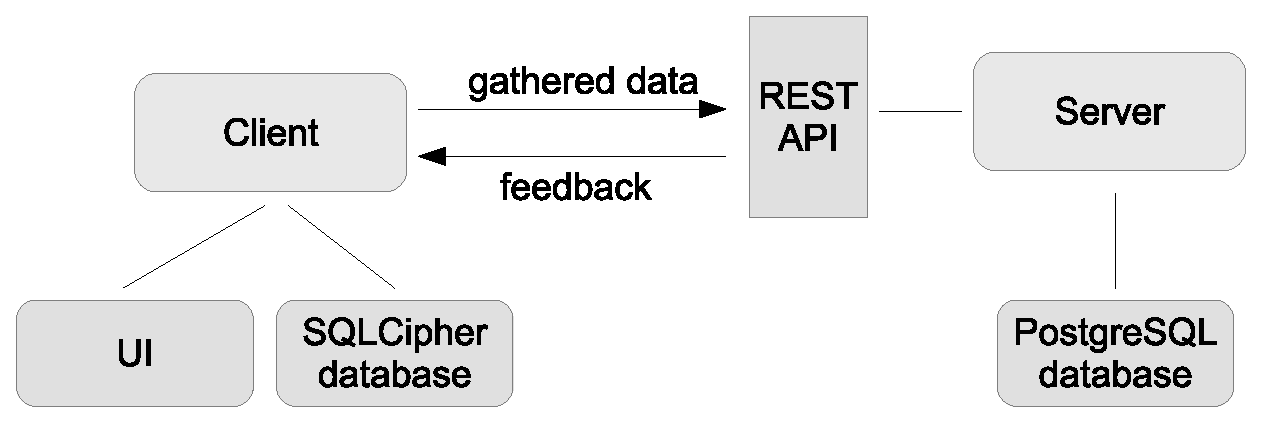
\includegraphics [width=0.7\textwidth]{images/Menthal_architecture}
  \caption{Menthal architecture}
  \label{fig:menthal_architecture}
\end{figure}

The client part consists of an Android application installed on a smartphone.
It keeps track of all the user activity during the day.
All the activities are stored as \textit{events}.
Each event contains such data as id, event type, timestamp, data itself and some additional information.
The main types of events are: SMS\_RECEIVED, SMS\_SENT, CALL\_RECEIVED, CALL\_OUTGOING, CALL\_MISSED, SCREEN\_UNLOCK, SCREEN\_LOCK, LOCALISATION.
The information gathering process is hidden from users, the application runs in the background, automatically sending data to the server.

The application gathers this data from different sources, using standard Android operating system API.
For example, to get the information about phone lock/unlock, it listens to the corresponding events and handles them.
To be aware of application usage, Menthal periodically (every 2 seconds) checks the current top application in the application stack of the smartphone.
If the application detects that the application has been changed, it writes the event into the database, adding a timestamp.
Catching a lock event is also used as a sign that the current application was changed and leads to a new record into the database.
The information about phone calls and sms can be queried from a local smartphone storage.
Every six hours Menthal checks whether the day is changed and if it does, it makes a new query to the local storage to get the latest information about performed calls and sent/received sms. 
 
\mnote{Menthal GUI}
Menthal has a user interface to provide users with a feedback. 
The main screen shows a 'score' - the relative phone usage measurement.
Using this value, one could check how intensively he uses his phone today comparing to previous days statistics.
UI provides also additional functionality.
It shows overall daily/weekly/monthly statistics about the phone usage such as most used application, number of calls or the number of times user unlocked the phone.
After a short questionary it can display personality characteristics diagram, that includes five sides: extraversion, neuroticism, openness, conscientiousness, agreeableness.
Furthermore a user can check the list of contacts with whom he communicates more often over a period of time.
The next screen shows the daily time spenditure with the phone for the last 30 days.
The application is able to keep track of user mood, periodically checking his current state of mind.
Using smartphone's GPS receiver, Menthal can determine and show on map the user location.
Moreover the application gives an opportunity to put a time limit on a particular application, so when the limit is exceeded the phone warns a user about that.

\begin{figure}[h]
\centering
\begin{minipage}{.5\textwidth}
  \centering
  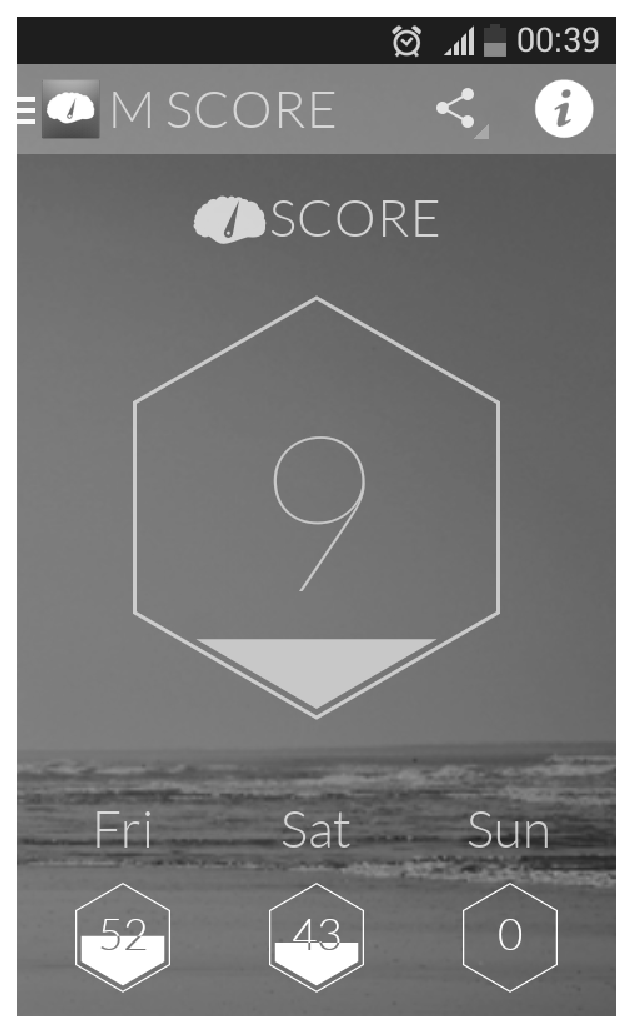
\includegraphics [width=.8\textwidth]{images/Menthal_GUI_mainscreen}
  \caption{Start screen}
  \label{fig:menthal_gui_mainscreen}
\end{minipage}%
\begin{minipage}{.5\textwidth}
  \centering
  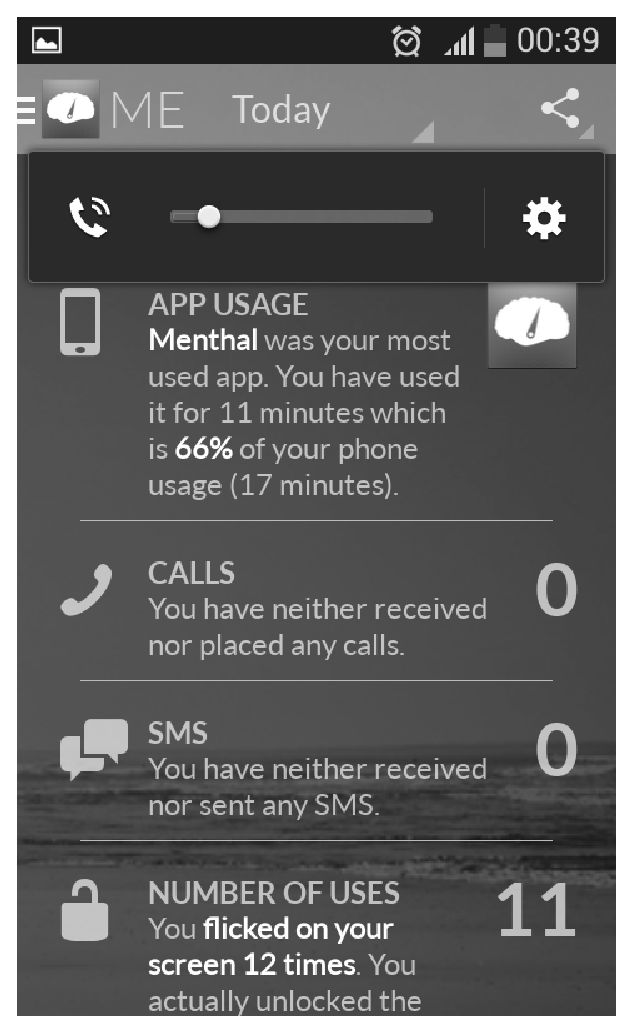
\includegraphics [width=.8\textwidth]{images/Menthal_GUI_me}
  \caption{Personal statistics}
  \label{fig:menthal_gui_me}
\end{minipage}
\end{figure}

\begin{figure}[h]
\centering
\begin{minipage}{.5\textwidth}
  \centering
  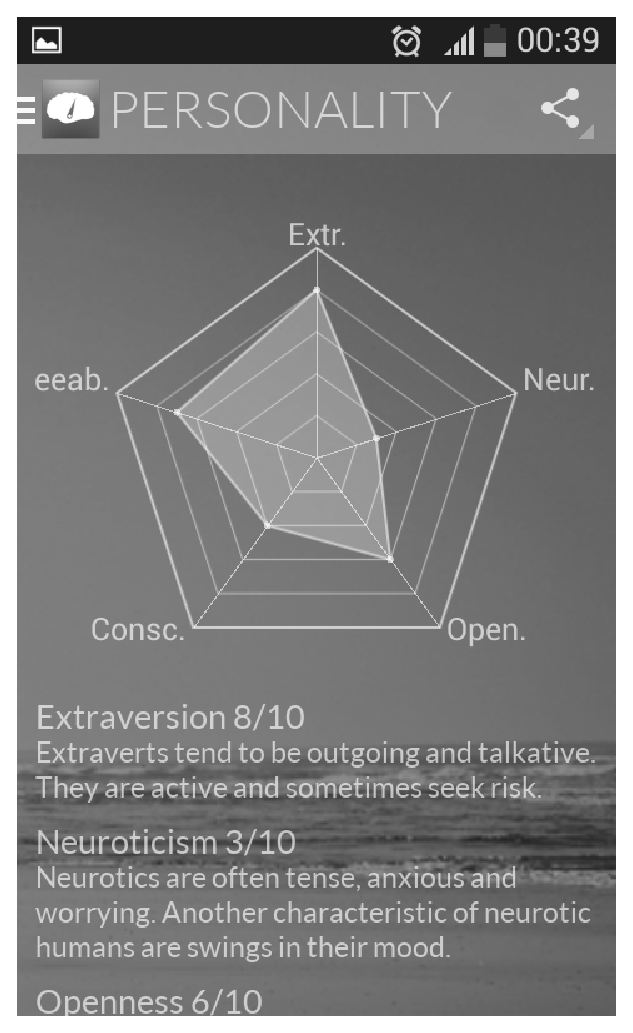
\includegraphics [width=.8\textwidth]{images/Menthal_GUI_personality}
  \caption{Personality characteristics}
  \label{fig:menthal_gui_personality}
\end{minipage}%
\begin{minipage}{.5\textwidth}
  \centering
  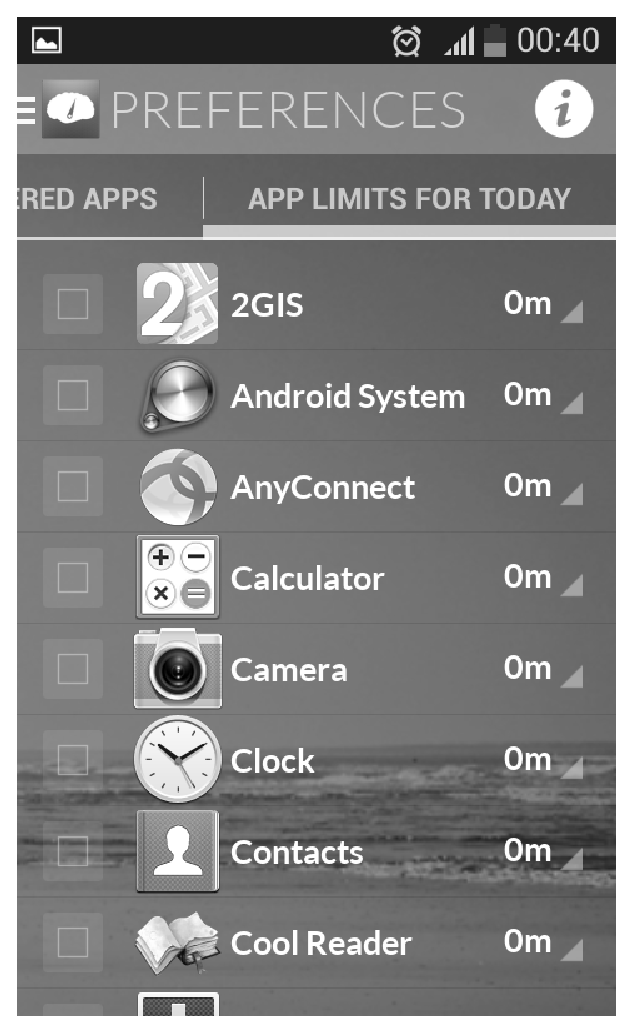
\includegraphics [width=.8\textwidth]{images/Menthal_GUI_preferences}
  \caption{Time limits preferences}
  \label{fig:menthal_gui_preferences}
\end{minipage}
\end{figure}

All the gathered data is temporarely stored on a phone in a cryptographically protected SQLCipher database.
Every time a new event is created, the application increases a special counter by 1.
When this value reaches 50, Menthal performs the following steps:

1) Obtain all the data from the SQLCipher database.

2) Convert it into JSON.

3) Send it to the server.

4) Wait for the reply.

5) If the server does not respose, try again in approximally 2 minutes. 

6) If the acknowledgment is received, delete the data that was sent from the SQLCipher database.

However, this is done only when a phone is connected to WiFi to avoid unnecessary charges for the user.
If the phone was not connected to WiFi during the day, Menthal still needs to send the data.
In this case the application sends it at random time between 1:00 - 6:00 at night via 3G.
All the data is sent in batches, where one batch contains no more than 50 events.

\mnote{information security}
Menthal uses secure connection, encryption of sensitive data and authentication mechanism to guarantee information security.
Communication between the client and the server goes through HTTPS.
This protocol is designed to provide a secure communication over a computer network. 
OAuth 1.0a protocol guarantees an authorization control.
When a client connects to the server the very first time, it receives a token.
Later the client sends this token with every message and the server uses it for authentication.
On the phone the data is stored in SQLCipher database.
This database uses 256 bit AES encryption for storing information in a secure way.
Moreover, Menthal hashes the sensitive data, such as the contact names or the phone numbers via SHA2. 

On the Server side Menthal has a cluster of 3 machines.
A PostgreSQL database is replicated between two of them.
One of these machines serves as a master node and another as a slave node.
The third machine hosts a key-value store that works as a read cache, message and task queues and a web application.
 
Menthal recently gained popularity among users.
It happened when the application was covered in mass media.
The articles in newspapers and interview with a project leader lead to the explosive increase of the number of users.
Almost 50 000 persons have this application installed on their phones.
All of these devices periodically send collected information to the server, that sums up to a vast amount of data.
Totally around 34Gb of information is received per day, that is almost 1Tb per month.
All these factors have a significant influence on the application performance.
The Menthal server side becomes overflowed and is not able to write all incoming data into database, not to mention providing a feedback.
Therefore, the application requires a new, enhanced server-side architecture that can meet the new requirements.
\chapter{Big Data Architecture [SP]}
\label{chap:big_data_architecture}

Traditionally, the process of making decisions is expensive and experiences significant error.
Simple reasoning is a straightforward approach, but it can work only till the certain point.
The main problem is that it can be easily ruined by the wrong assumptions.
Hence one would preferably use evidence based approaches that built on the accumulated data.
The most commonly used tools for this purpose are surveys and experiments, carried out on a control group.   
However, they both have significant disadvantages that makes the process of making decisions more complicated. 
On the one hand, surveys and experiments involve human resources, what leads to high expenses.
On the other hand, these approaches are also vulnerable to errors.
A lot of various reasons can cause an error, such as a survey composed in a wrong way, or a not representative control group.
 
Fortunately, this situation has changed dramatically in recent years.
First of all, data has become available for free, as a by-product of other processes (such as log files).
Moreover, constant reduction of data storage costs allows to warehouse enormous amounts of information, without troubling about the size limits.
Owing to the progress in the information technologies area, both transferring and processing of huge data volumes become easy.
All this gives us an alternative solution to the problem of making decisions that avoids the drawbacks of the strategies presented above.
The name of this solution is Big Data.

The main distinguishing feature of Big Data is that data collection is independent of use case.
Information is collected because it is available and cheap, with the hope that later on it can be used to answer a question that has not arisen yet.
For example, Facebook stores all available data about the users, like demographic information, geographic location, connections with other users, visited websites, clicked links, etc.
As a result it has a huge amount of data, which, with the right approach, can give lots of useful information. 
For instance, afterwards it can be used in targeted advertising, or for performing the social network analysis.

\section{Big Data}
\mnote{Big Data}
There is no consensus about the origins of the term "Big Data", but most of the sources claim that it is first mentioned in the press in 2008.
People start actively using it since 2009 and it spreads quickly owing to its precise and capacious meaning. 
Big Data is characterized by its high (i) variety, (ii) velocity and (iii) volume. [reference - find from wikipedia]
All these three "v" constitute a criterion that allocates Big Data observation into a distinct sector of computer science, which requires ad hoc decisions and a special approach.

\mnote{Variety}
First, Big Data sources are highly diverse.
They differ in the type of produced data - it can be text, images, sounds, raw feed incoming directly from sensors, etc.
Each of these types, in turn, may have a different format.
For instance, text can be transmitted in various languages, coding, formatting and so forth.
Big Data sources also differ in the speed of data flow and the data purity.  
Some of the sources generate noisy information, while others can produce data, that does not need cleaning.
Moreover, Big Data differ in the way how it is collected, how urgently it should be processed and which storage capabilities are available for its warehousing.

\mnote{Velocity}
The diversity of Big Data sources causes the high velocity of data input flow.
For example, Menthal, mentioned above, currently receives data from 50 000 users.
It sums up to almost 30Gb input data per day.
Therefore, Menthal reseives on average around 24Mb per minute, that sends a challenge how to handle input data flow on such a hight speed.

\mnote{Volume}
In the end, massive sources variety, multiplied by high velocity of data generation, results in its enormous size.
For instance, by the end of 2013, the number of Facebook users reaches 1.23 billion.
Each of them not only has some profile information, but also communicates with other users, shares data, updates the timeline and so forth.
In total 2.5 billion content items are shared every day.
Let us assume that each of these events is stored as a JSON object and needs 2Kb on average.
That means that in the end of the year Facebook deals with 4.65Tb * 365 = 1.65Pb of information.
And it is only metadata, not including images and video files that require significantly more space. 
As a result, Facebook deals with storing and processing petabytes of data.

Another example is the information received from sensors.
Sensor is a converter that measures and transforms physical quantity into a digital signal.
Sensors find an application in various fields: manufacturing industry, transportation systems, meteorology, medicine, even modern smartphones have lots of sensors.
The key feature of a sensor is that often it does its job constantly, continuously producing the flow of information, what leads to the large volumes of data.
Nest Labs is an American company that manufactures sensor-driven thermostats and smoke detectors.
The population of United States is about 318 million, so if every hundredth resident uses at least one of Nest thermostats in the house, it sums up to 3.2 million devices.
One thermostat has a variety of sensors, like activity, temperature, humidity, illumination, etc.
Each thermostat generates and transmits around 2Mb of data per day.
Consequently, all Nest thermostats in United States generate around 2.17Pb of data per year. 
The ability to process large amounts of information is the main benefit of Big Data analytics, since with its vast volume it is possible to construct better models.

\mnote{Batch Processing}
There are two fundamentally different ways of processing the Big Data, namely Batch and Real-Time data processing.
In the first case, data is handled in batches, i.e. process collects the data until the batch size is obtained, and only after this the process can perform the necessary actions on a batch as a whole.
This gives several advantages.
Batch processing can be done in the appropriate time, when the computing resources are less busy.
Furthermore, one can set a priority for each task, beginning with more urgent operations.
There is no need in a close supervision of a run, batch processing is mostly autonomous.
Finally, it becomes possible to process multiple operations in one request, instead of handling each operation individually.
That makes data treatment more efficient. 

To give a naive example how batching improves the performance, let us describe the problem of I/O operations.
For instance, an application every second receives data that should be written to the hard disk. 
There are two options how to implement the writing procedure.
On one hand, an application can write the input data every time it receives it, i.e. in our case every second.
On the other hand, it is possible to accumulate input data in memory until it reaches the defined size and than write the whole batch at a time.
It is known that I/O operations involve physical movement of mechanical devices (e.g. seek motion of hard drive).
Thus, the speed of sequential writes to a file is higher than random writes, because in the latter case additional time is spent for seek operations between each write.
This means that in our simple example the second option is preferable, because it decreses the number of seek operation and therefore makes the writing faster.    
The same principle also works in general case, i.e. combining multiple operations in one batch can significantly enhance performance.
However, Batch processing has one significant drawback: the results are always obtained with an arbitrary time delay.

\mnote{Real-Time Processing}
Real-time processing handles data at the moment of arrival. 
The advantage of the latter is that the results are ready almost immediately, which can be an essential requirement in such areas as medicine or security threat prediction. 
In spite of the fact that a certain delay is nevertheless exists, its duration is predetermine and is guaranteed to have a specified value.
That differentiates real-time processing from batch processing.
This fixed delay length varies depending on the application.
In some cases 10 minutes to perform all the computations is still considered to be a real-time processing.
However, in other cases, more than 1 second delay is unacceptable.
Real-time processing makes the information always available and up-to-date.

These significant advantages results in rising popularity of real-time processing, despite the fact that it requires greater effort to design and maintain.
Real-time processing can help to improve traffic in metropolitan areas, offering various travel alternatives for a vehicle, basing on analysis of incoming data about the situation on the roads.
Rapidity of data processing can be necessary in other cases as well.
Sometimes high processing speed can even be indispensable to life, when using in medicine, for example.
Special systems monitor the state of a patient, immediately alerting caregivers in the case of dangerous anomaly occurrence. 

\section{Architectural Requirements [SP]}

%System must provide information having gathered data from users and other sources.
%Application of complex algorithms is often necessary.
%Amount of data and rate of its arrival are heavy.
%Those aspects makes system to preprocess indices and aggregations that provide useful information.
%Batch processing is a good solution for that, nevertheless it has a drawback - execution time is long.
%Incremental processing resolves this issue.
%In combination these two approaches allow to design a system, that answers user queries with low latency as well as high accuracy.

%The purpose of the system is to answer queries having data.
%Let's consider an artificial example.
%Suppose we have a website where people pose programming questions, and other answer them.
%In this case the simplest query to the system is to return list of answers for a particular question post.
%Another query is to find all posts containing given keyword.

%One query is easy to answer, another requires application of complex algorithms.
%It is pretty easy to get list of answers to the question post having its id.
%You simply create hash-table that maps questions' ids to lists of answers' ids.
%Search by keyword, or even phrase search, is much more complex.
%To make it possibe we have to build specific inverted index, and this requires much more time to execute and to programm.
%Let's further assume, that our system has to provide keyword search, using precomputed inverted index. 

%Amount of data gathered with the time, as well as intense of arrival, can be huge.
%Let's consider again our example website.
%Assume that on average every second 5 questions and 20 answers appear.
%Every post is about 100 words, each of about 8 unicode symbols.
%The rate of incoming data is then $25*100*8*2=39$ KB per second.
%It is about 3.2 GB per day.
%This leads our system to be able to process such amount of data efficiently, as well as to rapidly reflect the state of inverted index with newly arrived posts.


There are some requirements that are common for most of the Big Data architectures.
Big Data systems deal with a large volumes of information, that constantly growth, therefore a system should be highly scalable.
Scalability has a direct impact on performance, thus it is essential to maintain a system performance on a proper level.
Moreover, availability and reliability are important attributes of a distributed architecture.
All these properties are described in the following paragraphs.

\mnote{Performance}
Performance is a quantitative characteristic of operation speed.  
This concept includes a variety of aspects, such as response time, processing speed, latency, bandwidth, etc.
With regard to extremely high volume and velocity of Big Data the question of system performance is a big issue.
For fair comparison of multiple systems performance a benchmark is used.
A benchmark is a sequence of tests that helps to estimate the performance of the system.

\mnote{Scalability}
Scalability indicates the property to handle an increasing amount of work.
It means that the performance of the system can be enhanced using additional hardware resources.
There are two types of scaling, namely vertical and horizontal.
Vertical scaling means that the single node of a system is enriched, e.g. CPU is added to a computer. 
Horizontal scaling denotes the enlargement of a system by adding new nodes.

\mnote{Commodity hardware}
In the context of Big Data architecture the latter method is of great interest for us.
First, in some cases the system should be distributed geographically.
For instance, adding new nodes closer to the customer can reduce the network load.
Second, because of the decreasing computer price it becomes possible to build highly performant systems using commodity machines.
A commodity computer is a moderately priced machine that is widely available for purchase.
The usage of inexpensive hardware helps considerably decrease the cost of the system.
It is especially relevant in the context of Big Data because of its overwhelming scales.
One of the well-known examples is the Google Lego server.
In 1996 two students, Larry Page and Sergey Brin, needed a cheap but capacious server to test the Pagerank algorithm on a huge data. 
[picture?]
They assembled it using 10 drives 4Gb each and a Lego enclosure. 
Nowadays Google uses commodity computers for building their computing clusters.

\mnote{Fault tolerance}
The direct consequence of the cheap hardware is the high failure rate.
Moreover, the large number of components also increases the probability of failure. 
Thus the system should be highly fault tolerant, with timely error detection and easy automatic recovery.

\mnote{Large files}
The world of Big Data introduces its own specific requirements for architecture design.
The file size can be enormous comparing to the standards.
It is not rare to work with a file of several gigabytes.
Storing the data in large files simplifies data processing.
The size of data itself is huge and it is more efficient to work with several large files than with great number of small files.

There are two metrics to measure the robustbness of a system, namely availability and reliability.
At first sight they look similar, however these two metrics assess a system from different perspective.
\mnote{Availability}
Availability means that a system operates properly at any given moment.
It can be calculated by the following formula: (total time - down time)/total time.
Consequently, availability depends on the sum of the time the system was down.
That means that even if the system fails every hour, but for negligible time, it is still considered to be highly available.

\mnote{Reliability}
In contrast, reliability denotes the capability of a system to operate continuously without failing.
Reliability and availability are the opposite concepts.
The highly available system mentioned above is not reliable, because the intervals of working without failing are relatively short.
However, the system that is down for one hour but only once per month can be reffered to sufficiently reliable.

Big Data architectures have to be targeted to each specific scenario.
For instance, architecture, designed for processing video data from a web camera, differs significantly from one for handling server log files.
Menthal, mentioned in Chapter 2, deals with data, that consists of a bulk of key/value pairs. 
As a result, Big Data technology becomes an umbrella of various systems. 
Data has to be collected, processed, transmitted, stored, protected from attacks, etc.

The Figure~\ref{fig:big_data_flow} shows the general flow of data within the Big Data concept.
Each of the presented steps involves a batch of technologies.
For example, depending on data type and size, one can choose SQL (MySQL, Oracle, Teradata, etc.) or NoSQL (Cassandra, MongoDB, Apache HBase, etc.) solutions for storing Big Data.
Similarly, depending on the application, Real-Time processing (Storm, Spark Streaming, etc.) or Batch processing (Apache Hadoop, etc.) technologies are used. 
Thereby, it is apparent that no one general solution exists for every Big Data problem.
Further we describe the existing Big Data architectures in the context of Menthal needs.

\begin{figure}
  \centering
  \includegraphics [width=0.8\textwidth]{images/big_data_flow}
  \caption{Big Data Flow}
  \label{fig:big_data_flow}
\end{figure}

\section{Naive Approach}
\mnote{PostgreSQL}
It is natural to start with a naive approach, using widely available and easy to use technologies.
As a storage system, one could use a relational database, such as MySQL or PostgreSQL.
PostgreSQL is an object-relational database management system.
It is an open source project, that is quite popular among developers due to its high security standards, good performance and scalability.
PostgreSQL was chosen as a database for Menthal application as a compromise between widespread but primitive MySQL and such large-scale solutions as Oracle or MongoDB.
On the one hand, it supports sufficiently complicated queries and easily scales, comparing to simple MySQL database.
On the other hand, it is not overload with redundant functional and does not require high maintenance affords as large-scale database management systems.

\mnote{REST}
Menthal uses a Representational state transfer (REST) API for communication between client and the database.
In this context RESTful API means that all the required information is transferred as parameters inside of an HTTP request (GET or POST).
The application uses stateless type of data exchange, that means that the server does not store a client state.
It helps to decrease the load on the server side, however increasing the amount of exchange traffic.
This straigforward approach is easy to implement, however, at a certain point, it cannot anymore sustain a constantly growing load.
The datatbase cannot cope anymore with the increased input flow, returning a timeout error.

\mnote{Database mirroring}
Database mirroring avoids the database overload.
It is a technique of keeping redundant copies of a database.
It enhances data availability and allows to always have an accessible copy of a database on one of the machines.
There is a special kind of mirroring called a hot standby, when every change is copied immediately to the mirrored instance.
In this case, there is a guarantee that all the instances keep the identical data, however, it can lead to a high latency.
If some data loss is permitted, a warm standby mode can be used, when the data is not fully synchronized across the database instances.
It does not grant the same information consistency as a hot standby mode, but it shows better performance results.

\mnote{Database caching}
Database caching is another technique for improving architecture scalability. 
In this case data is cached in high-performance store, e.g. in memory.
The access to memory is faster than the reading from a file or a database or transfering data via HTTP.
When the application often uses such external resources, database caching significantly increases performance. 
The drawback of both approaches is that they only improve reading, leaving the problem of large-scale writing unsolved. 

\mnote{Sharding}
In this situation it is reasonable to use horizontal partitioning, also known as sharding.
Sharding helps to enhance write scalability.
It denotes the process of partitioning of database tables by rows.
Each partition (shard) can be settled on separate machine.
This technology allows to spread the write load between multiple database servers.
Also it reduces the index size, thereby improving performance.
However, with growing input flow, the maintaining of shards and auxiliary infrastructure becomes more and more complex, demanding too much effort from developers. 	   
Hence the biggest IT corporations conduct their own research in this area, designing specific architectural solutions for working with Big Data.
\chapter{Lambda Architecture}
\label{chap:lambda_architecture}

The Lambda architecture \cite{MarzWarren201401} is a new solution
for creating a BigData system of any type. It provides the model for scalable,
fault-tolerant, distibuted processing of data. It uses both batch and online
processing to answer the queries. It provides human fault-tolerance, what is
often overlooked in other approaches. The Lambda architecture lets developer to
concentrate on the bussiness-logik, instead of thinking about distributing
computations, replication of dataset and how to manage intense grow of input data.

The core of the Lambda architecture is the equation "query = function(all
data)". The idea is that to answer any kind of query one can take the whole
dataset and execute particular function. The problem is that it is unreasonably
expensive, and even infeasible in most of cases. To solve this issue one can
create views, that are helpful for answeing particular queries, in advance. The
only problem of such approach is that indexing all the data and creating views
is high-latency operation. It can take several hours to be done. To overcome
this delay the Lambda architecture provides online processing of the data coming
in the real-time, that has not yet appeared in the precomputed views. As a
result, to answer the query both things are used: views, computed on the whole
dataset in advance, and sketch of the very new data.

One key aspect of the Lambda architecture, that makes a difference with the
other approaches, is that human fault-tolerance is concerned inherently. This is
important issue, because mistakes in programming code are guarantied. And as a
result, deleting or updating the data in a wrong way is also possible. The Lambda
architecture doesn't allow to modify data. This is called \mnote{Immutability}
immutability. Data can be only added, and never can be deleted or updated. This
leads to completely different model of storing data. Instead of having simple
tuple for a particular entity, every value of a tuple is stored separately and
has timestamp. Such technique allows to have the whole history of editions of
all attributes, what can be useful to make quesries that use history of changes.
At the same time the actual value is the one with the oldest timestamp.

\authorsection{General structure}{VI}

General view of the Lambda architecture is depicted on the
Figure~\ref{fig:lambda_architecture}. It consists of three main elements: batch
layer, serving layer and speed layer. Batch layer contains master dataset, that
allows only appending data. One executes computations on the whole master
dataset to obtain batch views, that are useful to answer queries. Serving
layer is the place where batch views are stored. It is also responsible for
providing interface for making particular queries from those views. Speed layer
provides temporal views. They contain sketches of data, that was obesrved during
ongoing batch processing in the batch layer. It is important, because batch
processing can last several hours or even longer. Speed layer is much more
complex than batch layer, and it provides only approximated results. We discuss
it in more details in the particular chapter.

\begin{figure}[H]
  \centering
  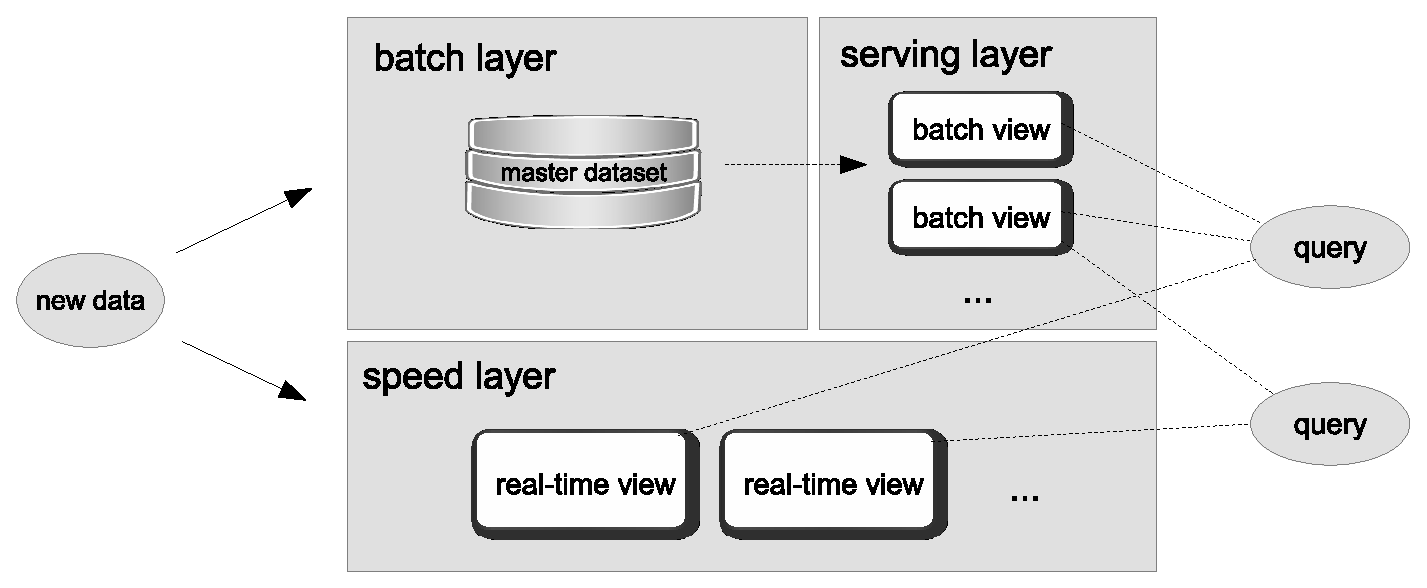
\includegraphics [width=0.9\textwidth]{images/LambdaArchitecture}
  \caption{General structure of the Lambda architecture}
  \label{fig:lambda_architecture}
\end{figure}

\authorsection{Batch layer}{VI}

Batch layer is the part of the Lambda architecture, that contains master dataset
and precomputes batch views, useful for answering queries. One can think about
master dataset as a very large list of records. This is of course simplified
representation, but for current discussion it is enough. When new piece of data
arrives to the system, it is being added to the master dataset. It can never
change old records, or cause deletion. This is what is called immutability of
data. This is a very important property, that provides human foult-tolerance,
and at the same time allows to execute queries on the whole history of changes.

Computation of batch views is being repeated continuously from scratch. This is
inherently distributed operation. That means that developer doesn't have to
think about concurrency and threads. He only wrties simple one-threaded code,
that is distributed than in the cluster. MapReduce is a perfect example of
a batch execution. Apache Hadoop is an example of framework that can be used for
computations in the batch layer.

\authorsection{Serving layer}{VI}

Serving layer is a place where batch views are loaded and indexed for very fast
access. It is represented by a specific distibuted database without ability to
make random writes. That simplifies things extremely, because opportunity
to make random writes brings most of complexity in databases. One example of
database that can be used for serving layer is ElephantDB.

\authorsection{Speed layer}{VI}


\chapter{Real time processing in Big Data context}
\label{chap:real_time_processing}

\authorsection{Something about Twitter}{NO}

\authorsection{Bloom filter, other algorithms}{NO}

\authorsection{Kafka paper}{NO}

\authorsection{Speed Layer (for real time processing)}{NO}
\chapter{Components}
\label{chap:components}

\authorsection{HDFS}{NO}

\authorsection{Storm}{NO}

\authorsection{Scala}{NO}

\authorsection{Redys}{NO}

\authorsection{Spark}{NO}

\authorsection{Alternatives}{NO}
\input{content/08-The_menthal_backend_architecture}
\chapter{Implementation}
\label{chap:implementation}

% rename chapter to Use cases

% first paragraph:
% architecture was described
% now we show how to use it
% two examples
% one subsection about aggregations
% one subsection about anomaly detection

Aggregations

In our project we use two types of aggregations: user-based and application-based.
Figure~\ref{fig:user_based_aggregations} represents the table of user-based aggregations.
Each of these aggregations is calculated with different granularities: hourly, daily, weekly and monthly.

\begin{figure}
  \centering
  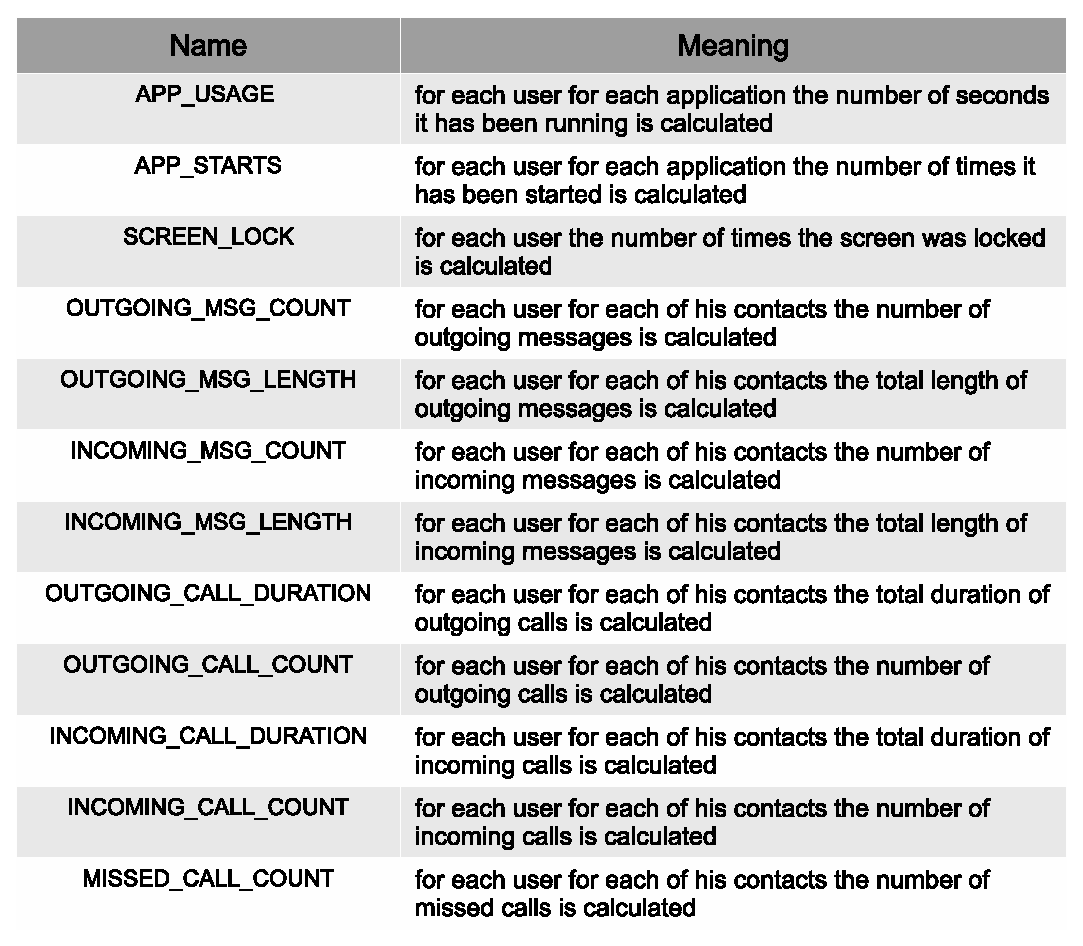
\includegraphics [width=1.0\textwidth]{images/user_based_aggregations}
  \caption{User-based aggregations}
  \label{fig:user_based_aggregations}
\end{figure}

The aggregations presented in the table are made for each user separately.
However, all these aggregations except SCREEN\_LOCK are also implemented as a sum and averadge for all users. 
Another group of aggregations is global summaries for different applications.
We calculate for each application the number of unique users, the number of sessions and total time spent. 

The implementation of aggregations in our case is based on Redis.
There is an interface \textit{EventAggregator} that actually allows to use any other data storages.
However, in our work we concentrate on Redis implementation of this interface.
It perfectly fits our needs for fast access and this storage is easy to use and does not need a lot of programming effort.


Anomaly Detection

People download various applications for their smartphones and do not pay much attention to the questions of security.
There is a risk that applications from unofficial stores contain the malicious software.
Moreover, the software from an official store can turn out to be infected.
The main problem is that usually users do not read what personal information the application requests an acces to.
And even if they read it, they do not have a choice to give the permissions or not.
Whithout giving the requred access rights, a user can not install this application on the smartphone.
   
The malicious software on smartphones behaves in different ways.
It can try to spread and infect all the contacts in a user's contact list.
For instance, a virus can send an sms, that contains its copy.
The virus can download and install another malicious software on the user's smartphone.
To apply some changes that the virus has performed in the system, it can restart the device.
Sometimes the malicious software can even make calls to specific numbers, so the user is charged for them.

\mnote{anomaly type}
As it was mentioned in Chapter , there are a lot of ways to detect anomaly in incoming data.
Let us first decide what kind of anomaly we are dealing with.
Ususally users do not have a strict pattern of interacting with their smartphones.
The sequence of performed actions changes from time to time.
One day a user can start with a phone call, another day by sending several messages.
This means that our anomaly is not \textit{collective}.
We consider a data instance independently from neighboring instances, therefore the anomaly type is not \textit{contextual}.
Thus we can conclude that we are dealing with the \textit{point} anomaly.

\mnote{anomaly detection approach}
Next step is to decide what approach to use for point anomaly detection.
The percentage of infected smartphones among the Menthal users is low.
It happens because the Android platform has good protection mechanisms and the official application stores are regularly tested for viruses.
Therefore we have a lot of \textit{normal} data and it is hard to get \textit{abnormal} examples (data from infected phones).
In this situation we can not use supervised learning, so we have chosen an unsupervised approach.

\mnote{One-class SVM}
There are several anomaly detection techniques that implement an unsupervised approach.
We decided to use one-class support vector machichenes (SVM) technique, because it perfectly fits our demands.
First, it needs only 'normal' data instances for learning.
Also it can work with high-dimension data, i.e. when a feature vector consists of more than two features (we need four in our case).
Moreover, there is an existing java library called libsvm [http://www.csie.ntu.edu.tw/~cjlin/libsvm/] that among other techniques implements one-class SVM.

Follow the assumed malicious software behavior, we try to detect the suspicious behavior of the smartphone.
For this purpose we analyze four events that are received from the clients: \textit{sms\_sent}, \textit{app\_install}, \textit{phone\_shutdown} and \textit{call\_outgoing}.
For simplicity we only count the number of these events.
However there is a possibility to make more thoroughtful research, using the values that these events contain.
For example, traffic data, namely the number of transferres bytes, can be used for analysis.
To have a basis for comparing the amount of events, we use a time window.
In other words, for each type of event we calculate the number of times it occures in a specified time interval (one hour by default).
Roughly speaking, we can take the number of times the event occures in a normal state, than calculate this number for an unknown state and make a conclusion whether it is normal or abnormal.

To use One-class SVM algorithm we need to create a training data set.
% TODO: write about training data

When the training set is ready we run \textit{svm\_train} method to create a model.
Then we use \textit{svm\_save\_model} method to safe the trained model, so it can be used later for anomaly detection.

\mnote{flow of events}
The Speed Layer has the following architecture to allow anomaly detection of incoming data.
Figure~\ref{fig:anomaly_detection_data_flow} illustrates the data flow.

\begin{figure}[h]
  \centering
  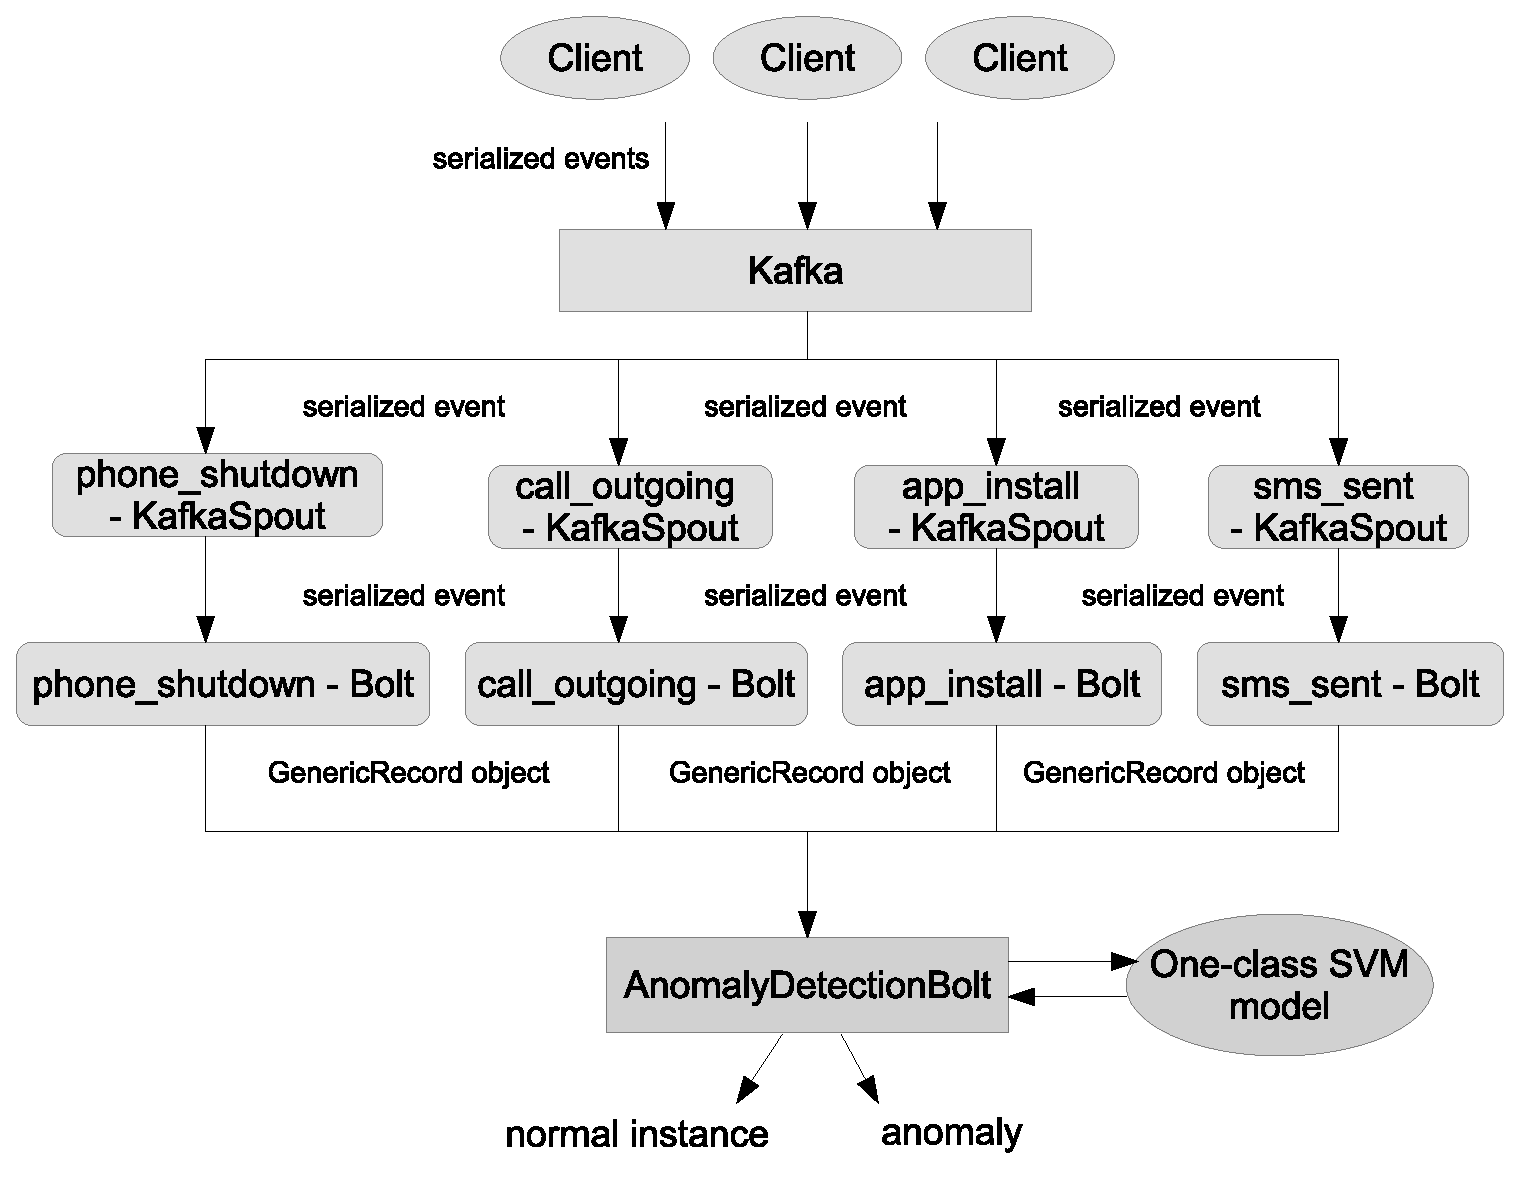
\includegraphics [width=1.0\textwidth]{images/anomaly_detection_data_flow}
  \caption{Anomaly detection: data flow}
  \label{fig:anomaly_detection_data_flow}
\end{figure}

For each Kafka topic a separate KafkaSpout receives messages.
One message contains the description of a particular event that happened on the client side (e.g. sms\_sent).
For each event type a separate bolt receives data from a corresponding KafkaSpout.
Then the bolt deserializes the received message, creating a \textit{GenericRecord} that represents the event.
For the events that are interesting for anomaly detection, there is an additional step.
Bolts, that receive data of type \textit{sms\_sent}, \textit{app\_install}, \textit{phone\_shutdown} and \textit{call\_outgoing}, emit the created GenericRecords to an \textit{AnomalyDetectionBolt}.

\mnote{Anomaly Detection bolt}
The main function of AnomalyDetectionBolt is to form data instances from incoming events.
As our version of Speed layer uses Redis as a data store, AnomalyDetectionBolt also uses it to accumulate events.
When a new event is received, AnomalyDetectionBolt extracts a type of event, a user id, and time when this event occured.
Using the user id, the bolt requests the value of \textit{lastCheckTime} that is stored in Redis.
The \textit{lastCheckTime} value is compared with the time, extracted from the received event.
If the time delta is bigger than a specified threshold, the new check for anomaly is performed.
The frequency of anomaly checks is regulated by an ANOMALY\_CHECK\_INTERVAL parameter.
This mechanism sets only one-side bound, so the check is performed not more than every half an hour by default.
However, if the bolt rare receives events from a particular user, the check for anomaly is run with the same low frequency. 

AnomalyDetectionBolt uses a sliding window to accumulate events.
The size of the window is regulated by a TTL parameter.
TTL specifies how long the event is stored in Redis.
Each time the new check for anomaly is performed, the bolt first of all deletes all outdated events from the store.
This guarantees that the data instance that participate in anomaly detection contains events that are collected over a specified period.
For example, the size of the sliding window is one hour by default.
If we want to perform an anomaly detection analysis, we take the mentioned earlier four types of events and count how many times each of them has occured during the last hour.
Using this numbers the bolt forms a data instance.  
Then it checks whether the instance is an anomaly or not using the trained one-class SVM model.

To get correct results it is essential to select the optimal parameters for One-class SVM.
Figure~\ref{fig:svm_parameters} represents the parameters, their meaning and values that are optimal for our case.
The process of parameters selection includes a technique called \textit{cross-validation}.
Here the data set is divided into two parts - training set and testing set.
This helps to avoid the problem of model overfitting.  

\begin{figure}[h]
  \centering
  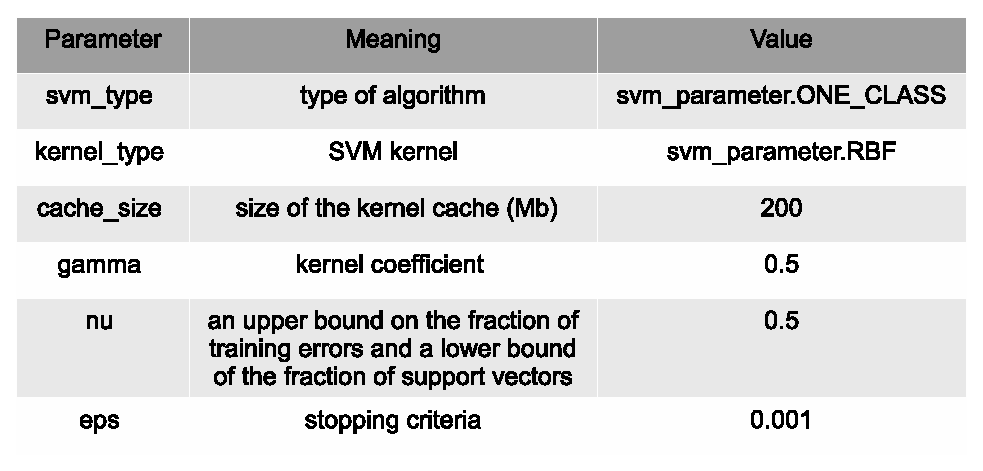
\includegraphics [width=0.9\textwidth]{images/svm_parameters}
  \caption{One-class SVM parameters}
  \label{fig:svm_parameters}
\end{figure}







 	

 
 

\input{content/10-Experiments}
\chapter{Summary}
\label{chap:summary}


%% Bibliographie
\backmatter
%\nocite{*}
\bibliography{bibliography/literature}

\appendix
\listoffigures
\listoftables
\lstlistoflistings

\end{document}
